% !TEX root = ../slides.tex
%%%%%%%%%%%%%%%%%%%%%%%%%%%%%%%%%%%%%%%%%%%%%%%%%%%%%%%%%%%%%%%%%%%%%%%%%%%%%%%%
% Session 7: Finite elements in d = 2
%%%%%%%%%%%%%%%%%%%%%%%%%%%%%%%%%%%%%%%%%%%%%%%%%%%%%%%%%%%%%%%%%%%%%%%%%%%%%%%%

\session{session07}{The finite-elements method}{Finite elements in \texorpdfstring{$d=2$}{d=2}}
{Chapter 4}
{\notebook{lectures/finite-elements/d-greater-1}{FEMlinear2dLaplaceDirichlet.ipynb}}
{--}

\begin{frame}{Plan for today}
    \begin{enumerate}
        \item A zoo of elements in $d = 2$: triangles and rectangles.
        \item The Dirichlet Laplacian with piece-wise linear functions.
        \item Uniform square triangulation: back to finite differences.
        \item General triangulations: computing the matrices.
    \end{enumerate}
    \bigskip
    \textbf{Notation.} $\R_k[x,y]$: polynomials of degree $\le k$ in two variables, \ $\dim \R_k[x,y] = \frac{(k+1)(k+2)}{2}$.
    \medskip

    Triangle with non-collinear vertices $z_1, z_2, z_3$:
    \[
        \trianglegenerated(z_1,z_2,z_3) = \Big\{ \sum_{i=1}^3 \theta_i z_i : \theta_i > 0,\ \sum_{i=1}^3 \theta_i = 1 \Big\}
    \]
    ($\theta_i$ are the \emph{barycentric coordinates}).
\end{frame}

\begin{frame}{Lagrange triangles}
    \begin{columns}[T]
        \begin{column}{.48\textwidth}
            \textbf{Linear Lagrange triangle}
            \begin{itemize}
                \item $\mathcal P = \R_1[x,y]$ ($\dim = 3$),
                \item $N_i(v) = v(z_i)$, $i = 1,2,3$ (vertices).
            \end{itemize}
            On the reference triangle $z_1 = (0,0)$, $z_2 = (1,0)$, $z_3 = (0,1)$:
            \[
                \psi_1 = 1 - x - y, \quad \psi_2 = x, \quad \psi_3 = y.
            \]
        \end{column}
        \begin{column}{.48\textwidth}
            \textbf{Quadratic Lagrange triangle}
            \begin{itemize}
                \item $\mathcal P = \R_2[x,y]$ ($\dim = 6$),
                \item $N_i(v) = v(z_i)$: vertices $z_1,z_2,z_3$ and mid-points of the edges
                      $z_4 = \frac{z_2 + z_3}{2}$, $z_5 = \frac{z_1 + z_3}{2}$, $z_6 = \frac{z_1 + z_2}{2}$.
            \end{itemize}
        \end{column}
    \end{columns}
    \begin{center}
        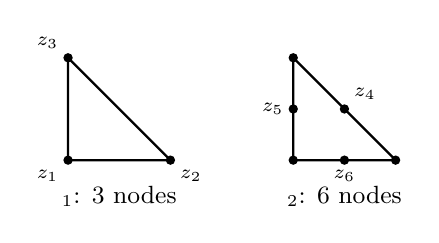
\begin{tikzpicture}[scale=1.3]
            \draw[thick] (0,0) -- (1,0) -- (0,1) -- cycle;
            \foreach \p/\l/\a in {{(0,0)}/z_1/below left, {(1,0)}/z_2/below right, {(0,1)}/z_3/above left}
            \fill \p circle (1.3pt) node[\a] {\scriptsize $\l$};
            \node at (.5,-.35) {\small $\R_1$: 3 nodes};
            \begin{scope}[xshift=2.2cm]
                \draw[thick] (0,0) -- (1,0) -- (0,1) -- cycle;
                \foreach \p in {(0,0),(1,0),(0,1),(.5,.5),(0,.5),(.5,0)} \fill \p circle (1.3pt);
                \node[above right] at (.5,.5) {\scriptsize $z_4$};
                \node[left] at (0,.5) {\scriptsize $z_5$};
                \node[below] at (.5,0) {\scriptsize $z_6$};
                \node at (.5,-.35) {\small $\R_2$: 6 nodes};
            \end{scope}
        \end{tikzpicture}
    \end{center}
    \board{why is the glueing continuous? On an edge, $v \in \R_k$ is a polynomial of degree $k$ in one variable, determined by its values at the $k+1$ nodes of the edge.}
\end{frame}

\begin{frame}{Cubic Hermite triangle and rectangles}
    \small
    \begin{columns}[T]
        \begin{column}{.5\textwidth}
            \textbf{Cubic Hermite triangle}
            \begin{itemize}
                \item $\mathcal P = \R_3[x,y]$ ($\dim = 10$),
                \item values at the vertices and the centroid $z_4$ (4),
                \item both first derivatives at the vertices (6).
            \end{itemize}
            \textbf{Bi-linear rectangle} $K = (0,1)^2$
            \begin{itemize}
                \item $\mathcal P = \mathbb Q_1 = \spannedby\{1, x, y, xy\}$,
                \item values at the 4 corners.
            \end{itemize}
            \textbf{Bi-quadratic rectangle}
            \begin{itemize}
                \item $\mathcal P = \mathbb Q_2 = \spannedby\{x^iy^j : 0 \le i,j \le 2\}$,
                \item values at corners, mid-points of sides and centre (9).
            \end{itemize}
        \end{column}
        \begin{column}{.46\textwidth}
            \centering
            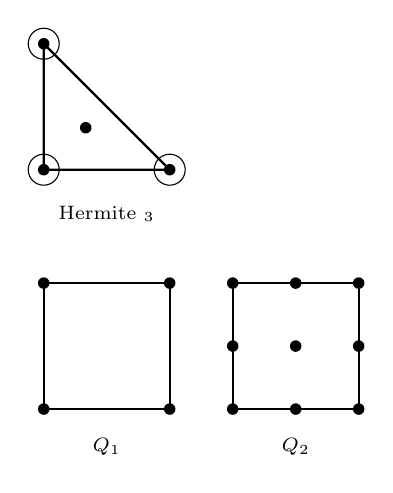
\begin{tikzpicture}[scale=1.6]
                \draw[thick] (0,0) -- (1,0) -- (0,1) -- cycle;
                \foreach \p in {(0,0),(1,0),(0,1)} {\fill \p circle (1.3pt); \draw \p circle (3.5pt);}
                \fill (1/3,1/3) circle (1.3pt);
                \node at (.5,-.35) {\scriptsize Hermite $\R_3$};
                \begin{scope}[yshift=-1.9cm]
                    \draw[thick] (0,0) rectangle (1,1);
                    \foreach \p in {(0,0),(1,0),(0,1),(1,1)} \fill \p circle (1.3pt);
                    \node at (.5,-.3) {\scriptsize $\mathbb Q_1$};
                \end{scope}
                \begin{scope}[xshift=1.5cm,yshift=-1.9cm]
                    \draw[thick] (0,0) rectangle (1,1);
                    \foreach \x in {0,.5,1} \foreach \y in {0,.5,1} \fill (\x,\y) circle (1.3pt);
                    \node at (.5,-.3) {\scriptsize $\mathbb Q_2$};
                \end{scope}
            \end{tikzpicture}

            {\scriptsize dot: value; circle: first derivatives}
        \end{column}
    \end{columns}
    \medskip
    \textbf{B-splines} on uniform meshes: tensor products $b_{p,i,h}(x)\, b_{p,j,h}(y)$.
\end{frame}

\begin{frame}{Many more elements}
    \centering
    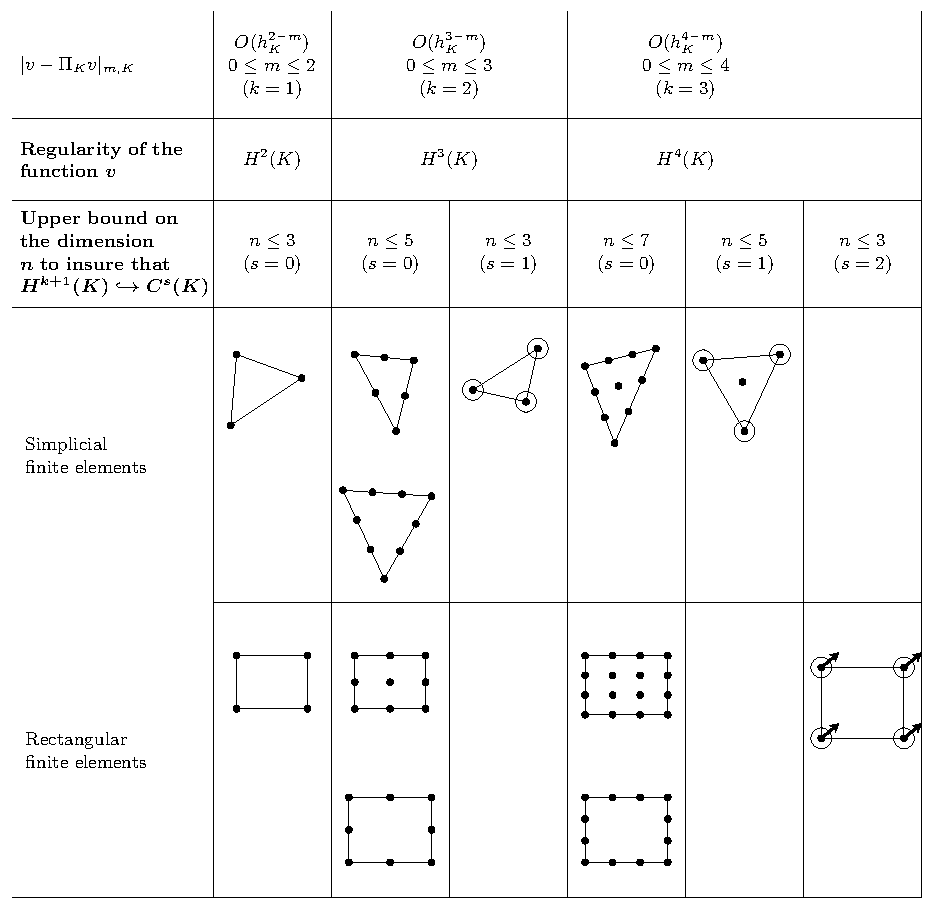
\includegraphics[height=.78\textheight]{../../lectures/finite-elements/d-greater-1/Ciarlet_diagram.pdf}

    {\scriptsize Reproduction of Figure 3.1.2 in Ciarlet, \emph{The Finite Element Method for Elliptic Problems}. Dot: evaluation; circle: also first derivatives.}
\end{frame}

\begin{frame}{The Dirichlet Laplacian with piece-wise linear functions}
    \small
    Triangulation $\mathcal T$ of $\Omega$ with vertices $x_i$; for each $K \in \mathcal T$ an affine map $F_K: K_0 \to K$ from the reference triangle.
    \medskip

    \textbf{Global basis.} $\varphi_i$ continuous, linear on each triangle, $\varphi_i(x_j) = \delta_{ij}$:
    \[
        \varphi_i\big|_K =
        \begin{cases}
            \psi_j \circ F_K^{-1} & \text{if } x_i = F_K(z_j) \text{ is a vertex of } K, \\
            0                     & \text{if } x_i \notin \overline K.
        \end{cases}
    \]
    \begin{itemize}
        \item $\varphi_i$ is continuous across edges (linear on each edge, same values at the vertices), so $\varphi_i \in H^1(\Omega)$ by the glueing theorem.
        \item Dirichlet conditions: basis of $\mathcal P_{\mathcal T} \cap H^1_0(\Omega)$ is $\{\varphi_i : x_i \in \Omega\}$ (interior vertices).
        \item Stiffness matrix:
              \[
                  \int_\Omega \nabla\varphi_i \cdot \nabla \varphi_j = \sum_{K:\ x_i, x_j \in \overline K} \int_K \nabla \varphi_i\cdot\nabla\varphi_j .
              \]
              Zero unless $x_i$ and $x_j$ share a triangle: \alert{sparse} matrix. $\nabla\varphi_i$ is constant on each $K$.
    \end{itemize}
\end{frame}

\begin{frame}{Uniform square triangulation}
    $\Omega = (0,1)^2$, $h = 1/N$, nodes $x_{ij} = (ih, jh)$; each square is cut along a diagonal.
    \begin{columns}[c]
        \begin{column}{.32\textwidth}
            \centering
            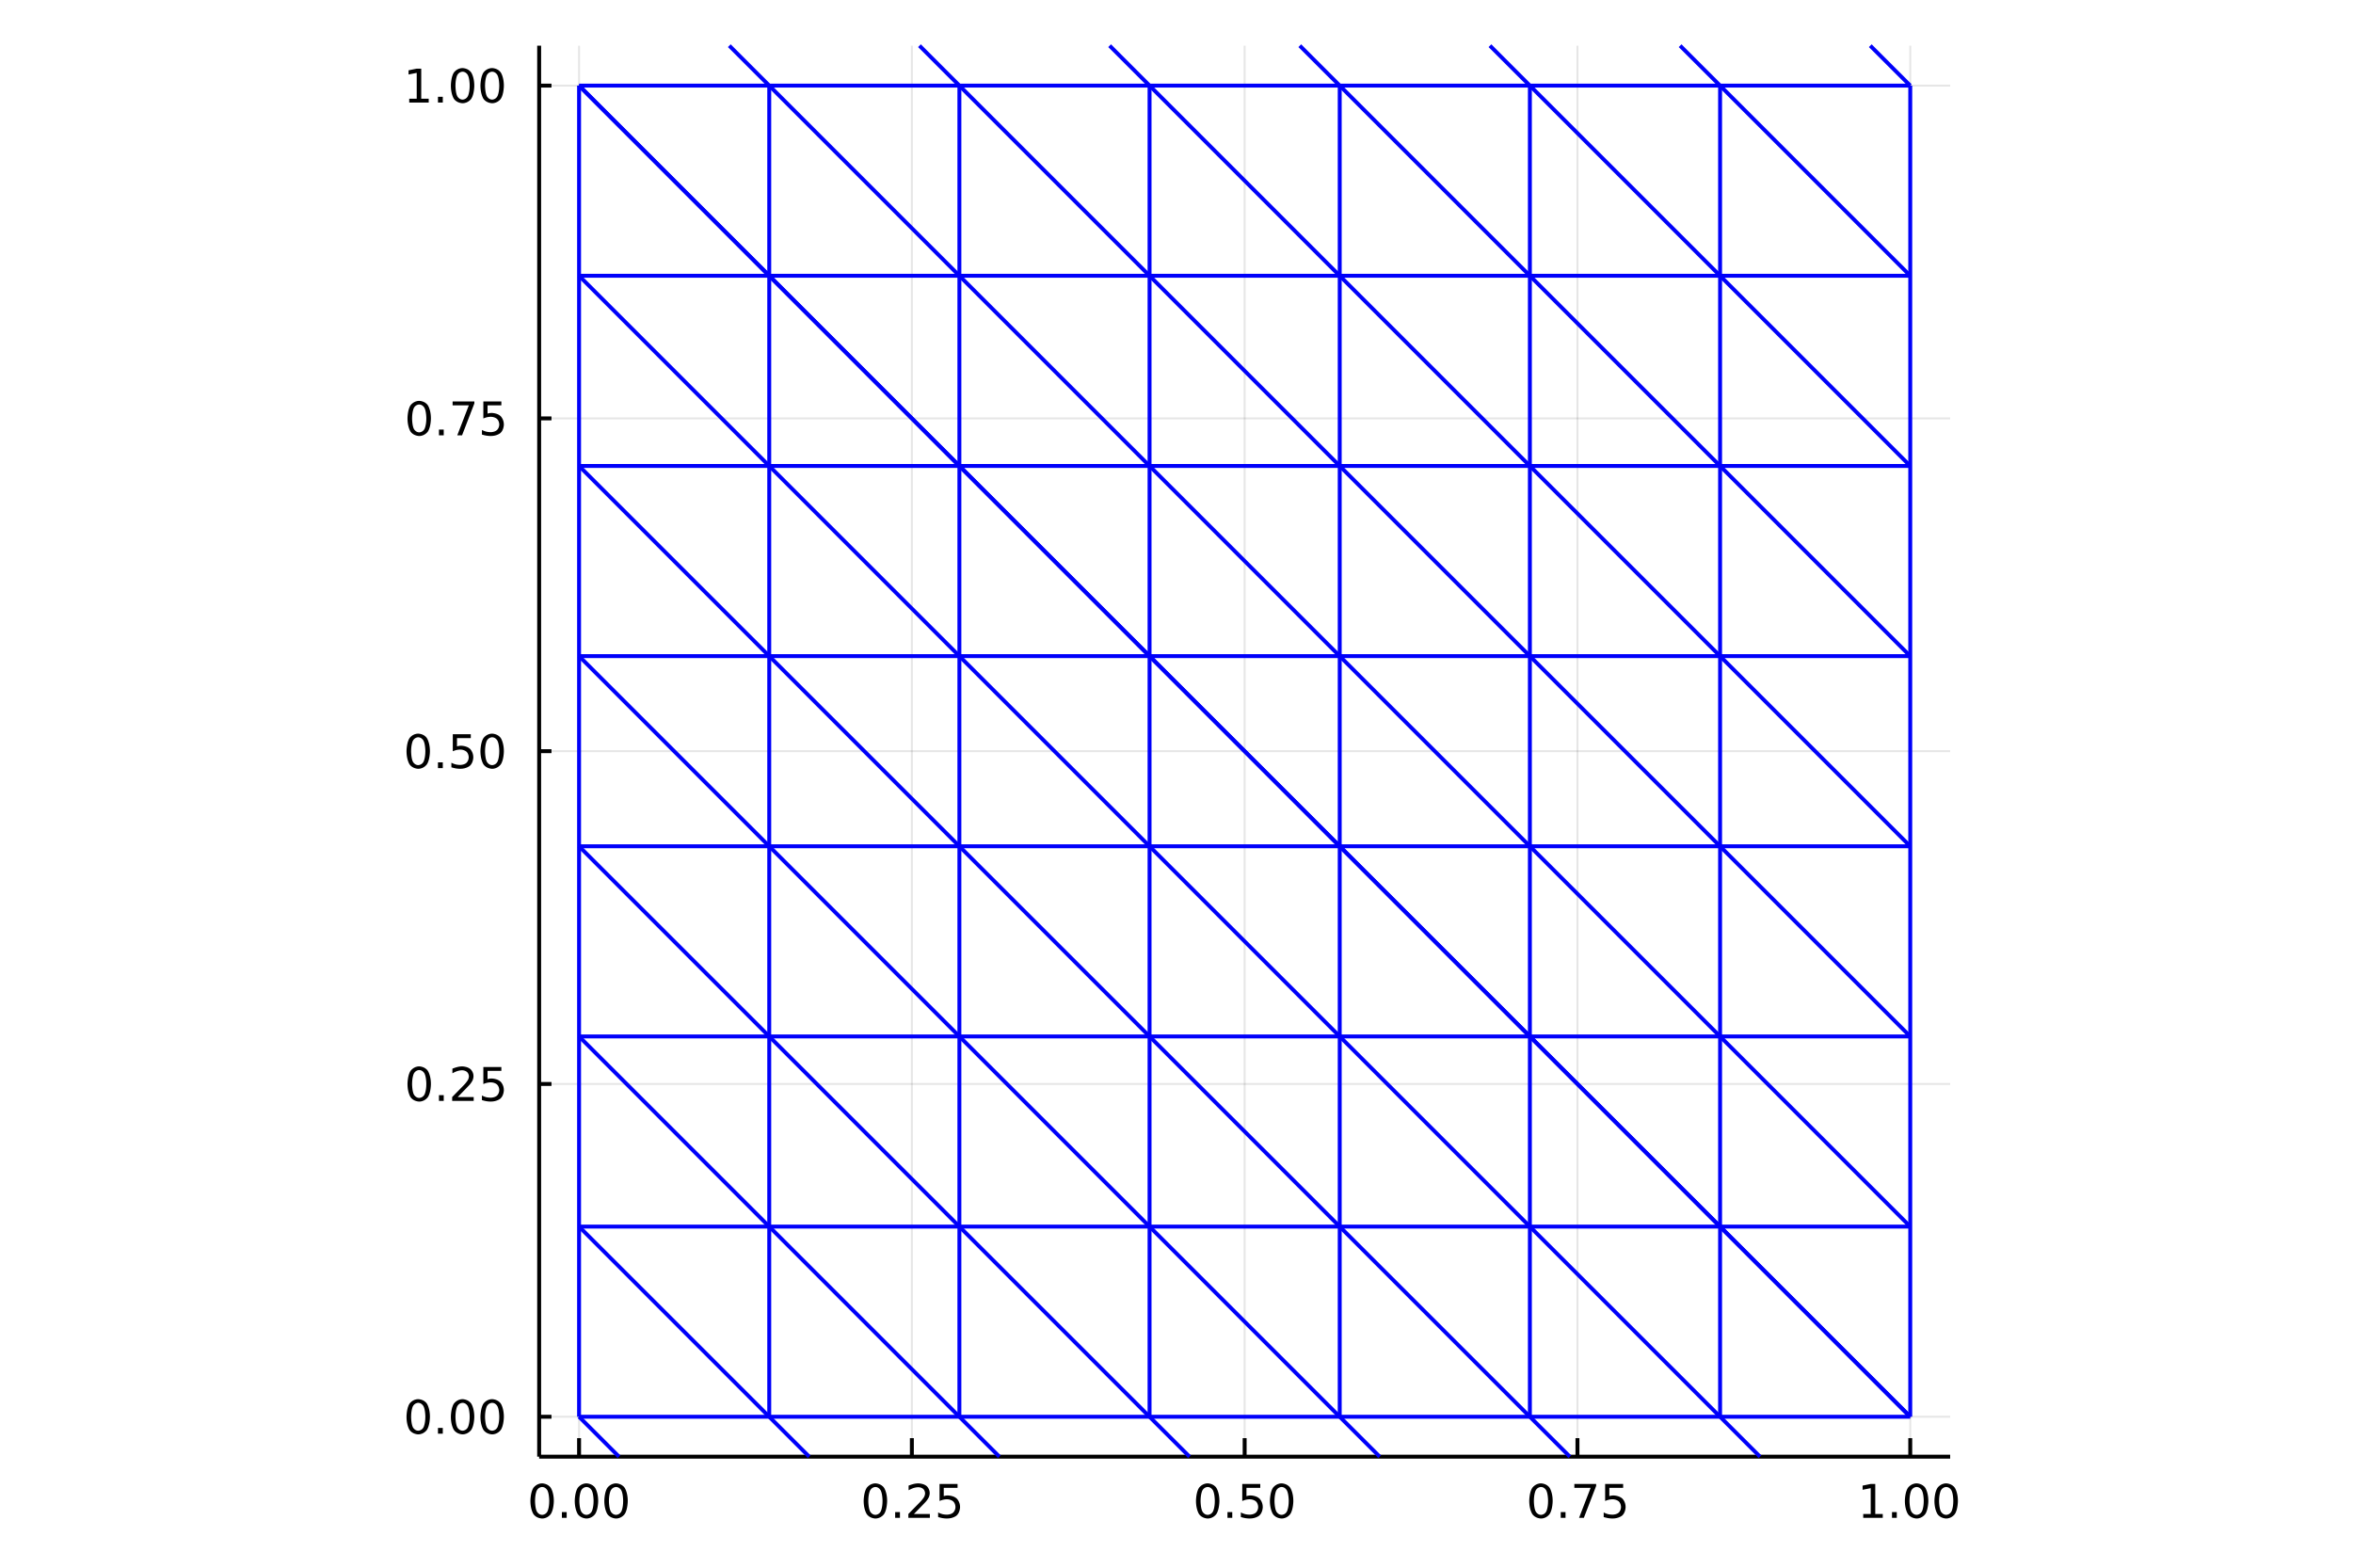
\includegraphics[width=\textwidth]{../../lectures/finite-elements/d-greater-1/UniformMesh.png}

            {\scriptsize triangulation}
        \end{column}
        \begin{column}{.25\textwidth}
            \centering
            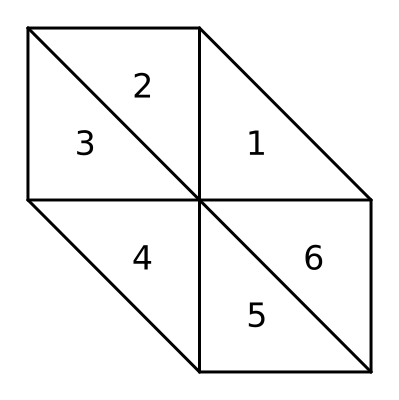
\includegraphics[width=\textwidth]{../../lectures/finite-elements/d-greater-1/UniformMesh2.png}

            {\scriptsize the 6 triangles around $x_{ij}$}
        \end{column}
        \begin{column}{.38\textwidth}
            \centering
            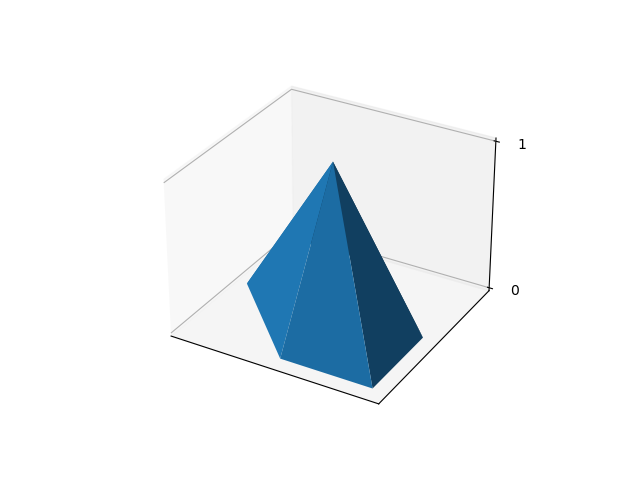
\includegraphics[width=\textwidth]{../../lectures/finite-elements/d-greater-1/Piramid.png}

            {\scriptsize $\varphi_{ij}$: a pyramid}
        \end{column}
    \end{columns}
    \medskip
    On each of the six triangles, $\varphi_{ij}$ is one of
    \[
        1 - \tfrac{x - x_i}{h} - \tfrac{y - y_j}{h},\quad
        1 - \tfrac{y - y_j}{h},\quad
        1 - \tfrac{x_i - x}{h},\quad
        1 - \tfrac{x_i - x}{h} - \tfrac{y_j - y}{h},\quad
        1 - \tfrac{y_j - y}{h},\quad
        1 - \tfrac{x - x_i}{h}.
    \]
\end{frame}

\begin{frame}{Back to finite differences}
    Galerkin approximation of $-\Delta u = f$ in $(0,1)^2$, $u = 0$ on $\partial\Omega$:
    \[
        u_h = \sum_{k,l = 1}^{N-1} U_{kl}\, \varphi_{kl},
        \qquad
        \sum_{k,l} U_{kl} \iint_\Omega \nabla \varphi_{kl} \cdot \nabla \varphi_{ij} = \iint_\Omega f \varphi_{ij}.
    \]
    \board{compute the integrals: only the neighbours $(i\pm1, j)$, $(i, j\pm1)$ survive.}
    \[
        \frac{-U_{i+1,j} + 2U_{ij} - U_{i-1,j}}{h^2} + \frac{-U_{i,j+1} + 2U_{ij} - U_{i,j-1}}{h^2}
        = \frac{1}{h^2} \iint_{\supp\varphi_{ij}} f\, \varphi_{ij} .
    \]
    \begin{itemize}
        \item This is the \alert{five-point finite-difference scheme} (with an averaged right-hand side).
        \item In matrix form: Kronecker products of the $1$-dimensional finite-difference matrix.
        \item The finite-element framework works on any triangulation, not only on uniform grids.
    \end{itemize}
\end{frame}

\begin{frame}{General triangulations: direct computation}
    On a triangle with vertices $P = (x_1,y_1)$, $Q = (x_2,y_2)$, $R = (x_3, y_3)$, the linear function with values $1, 0, 0$ is
    \[
        \varphi(x,y) = 1 + \frac{y_2 - y_3}{D}(x - x_1) + \frac{x_3 - x_2}{D}(y - y_1),
    \]
    \[
        D = (x_2 - x_1)(y_3 - y_1) - (y_2 - y_1)(x_3 - x_1) \qquad (|D| = 2|K|).
    \]
    \begin{itemize}
        \item $\nabla\varphi = \frac{1}{D}(y_2 - y_3,\ x_3 - x_2)$ is constant: $\int_K \nabla\varphi_i\cdot\nabla\varphi_j = |K|\, \nabla\varphi_i\cdot\nabla\varphi_j$.
        \item The area can also be computed with Heron's formula:
              $|K| = \sqrt{s(s-a)(s-b)(s-c)}$, \ $s = \frac{a+b+c}{2}$.
    \end{itemize}
    \board{Exercise 2.4: write the local stiffness matrix of a triangle in terms of its edge vectors.}
\end{frame}

\begin{frame}{General triangulations: via the reference triangle}
    \small
    If $F_K(z_{j_k}) = x_{i_k}$, change variables $x = F_K(\widehat x) = \mat A_K \widehat x + \vec b_K$:
    \begin{align*}
        \int_K \varphi_{i_1}\varphi_{i_2}                         & = |\det \mat A_K| \int_{K_0} \psi_{j_1}\psi_{j_2},                                                            \\
        \int_K \nabla\varphi_{i_1}\cdot\nabla\varphi_{i_2} & = |\det \mat A_K| \int_{K_0} \big(\mat A_K^{-t}\widehat\nabla\psi_{j_1}\big)\cdot\big(\mat A_K^{-t}\widehat\nabla\psi_{j_2}\big).
    \end{align*}
    \begin{example}[Local mass matrix of the linear triangle]
        \textcolor{mnuaccent}{\textbf{Check it at the board:}} \quad
        $\Big(\int_{K}\varphi_{i_a}\varphi_{i_b}\Big)_{a,b=1}^3 = \frac{|K|}{12}\left(\begin{smallmatrix} 2 & 1 & 1 \\ 1 & 2 & 1 \\ 1 & 1 & 2 \end{smallmatrix}\right).$
    \end{example}
    \textbf{Assembly} (as in $d=1$; it extends to other elements and to $d = 3$):
    \begin{enumerate}
        \item connectivity table: the three global vertex indices of each triangle;
        \item loop over the triangles: compute the $3\times3$ local matrices and add them to the global matrix;
        \item remove the boundary vertices (Dirichlet conditions).
    \end{enumerate}
\end{frame}

\begin{frame}{Summary and practice}
    \begin{itemize}
        \item Elements in $d=2$: Lagrange triangles ($\R_k$), Hermite triangle, rectangles ($\mathbb Q_k$), tensor B-splines, \dots
        \item Linear triangles: global hat functions (pyramids), sparse stiffness matrix.
        \item Uniform triangulation of the square: five-point finite-difference scheme.
        \item General meshes: compute on each triangle (directly or via $K_0$) and assemble.
        \item Error (shape-regular meshes, $u \in H^2$): $O(h)$ in $H^1$ and $O(h^2)$ in $L^2$ (Session 5).
    \end{itemize}
    \bigskip
    \textbf{Practice.}
    \begin{itemize}
        \item Notebook \notebook{lectures/finite-elements/d-greater-1}{FEMlinear2dLaplaceDirichlet.ipynb}.
        \item Solve $-\Delta u = f$ on a non-uniform triangulation and check the rates of convergence.
    \end{itemize}
    \bigskip
    \textbf{Next session:} spectral methods.
\end{frame}
